\documentclass[12pt]{article}
\usepackage{graphicx} % Required for inserting images
\usepackage{fontspec}
\usepackage{unicode-math}
\usepackage[style=numeric,url=false,isbn=false]{biblatex}
\usepackage{amsmath}
\usepackage{listings}

\addbibresource{Coupling.bib}
%\addbibresource{Fusion_WDMApp.bib}
\setmainfont{Times New Roman}

\title{PCMS: Parallel Coupler for Multimodel Simulations}
\author{Jacob Merson, Cameron Smith, Mark S. Shephard}
\date{April 2023}

\usepackage{draftwatermark}
\SetWatermarkText{DRAFT}
\SetWatermarkScale{1}

\begin{document}

\maketitle
\section{Coupler Design}
test pdf compile

% C++ interface supports an "open set" of mesh types
\subsection{Background}
PCMS is a library that is designed to make in-memory tight coupling a range of large scale parallel simulation codes as easy as possible without modification of their internal data-structures or algorithms and without making compromises with respect to efficiency or accuracy. It is focused on multimodel simulations, which encompasses both partitioned multiphysics analysis as well as concurrent and hierarchical multiscale analysis.

To support the broadest set of codes, we have developed the following set of design requirements 
\begin{itemize}
    \item Does not modify existing datastructures or computational algorithms in the simulation codes.
    \item Makes efficient use of the largest supercomputers available (today, exascale).
    \item Efficiently handles data and coordinate transformations.
    \item Performs efficient operations with the complete range of structured and unstructured meshes.
    \item Handles parallel coordination and communication of distributed field data.
\end{itemize}

The combination of three components sets PCMS apart from the other coupling efforts: 1) Integration of coordinate and data transformations. 2) Parallel control and transfer algorithms for fields on structured and unstructured meshes. 3) Focus on ease of use and limiting the need for intrusive code changes. 4) Use of an intermediate data representation when direct coupling is not possible to avoid quadratic growth of coupling implementations.

One of the motivating use cases for PCMS is to support Tokamak coupling. Many of the codes associated with Tokamaks use specialized physics based coordinate systems that follow the magnetic field lines. These coordinate systems are not unique, so codes take advantage of those that make their computational methods more efficient. From a design perspective, this implies that we need to be able to handle an open set of coordinate systems.


\subsection{Review of Existing Coupling Codes}
The well versed reader will recognize that individually some of these components are available in existing software. However, it is the combination of the four components and the strict adherence to our design requirements that sets PCMS apart. The following section will provide a brief description of other existing coupling tools.


\begin{itemize}
    \item Moose: intrusive/monolithic solver \cite{gastonMOOSEParallelComputational2009}
    \item preCICE: easy to user interface, uses RBF for field transfer, no coordinate system support, no mesh based field support. Currently unsure about scalability...need to search through papers. \cite{bungartzPlugandplayCouplingApproach2015,bungartzPreCICEFullyParallel2016,chourdakisPreCICEV2Sustainable2022}.
    \item DTK: implemented rendevouz algorithm, no support for coordinate systems, focusses solely on field transfer part of coupling \cite{slatteryDataTransferKit2013}, no scalability results for current supercomputers (with GPUs) found, although they do seem to have concept of memory space in current API. developed as part of CASL. Requires Trilinos
    \item MPCCI: commercial code requires license, no indication that it can work with supercomputers as it is focused on coupling commercial codes \cite{joppichMpCCIToolSimulation2006, mehlParallelCouplingNumerics2016}
    \item Integrated Plasma Simulator (IPS)/ One Modeling Framework for Integrated Tasks (OMFIT) File based, freeform treelike structure, coupling through application native "datastructures" (file-io), contend that only a few pairs of well defined codes will ever need to be coupled, so no need to worry about the \(n^2\) problem of letting \(n\) independent formats couple \cite{foleyIntegratedPlasmaSimulator2011,meneghiniIntegratedModelingApplications2015}
    \item Integrated Modeling and Analysis System (IMAS), standard fileformat/layout developed by ITER for experimental and simulation data. Not clear that this can/should be used for tight coupling \cite{romanelli2020code}.
    \item European Transport Simulator (ETS) \cite{kalupinNumericalAnalysisJET2013, costerBuildingTurbulencetransportWorkflow2021}
\end{itemize}


%\subsection{Terminology}
%The following is a few bits of terminology that are useful to understand with respect to the design of 
%Open-closed principle...open for extension, closed for modification
%\begin{itemize}
%    \item \textbf{Open Set of Types}: 
%    \item \textbf{Closed Set of Types}:
%    \item \textbf{Customization Point}:
%    \item \textbf{Type Erasure}:
%\end{itemize}
%
%Field types are open set
%Datatype of underlying data in field is closed set (restriction imposed by communication layers
%Need to discuss type safety

\subsection{Design}
\begin{figure}[ht]
    \centering
    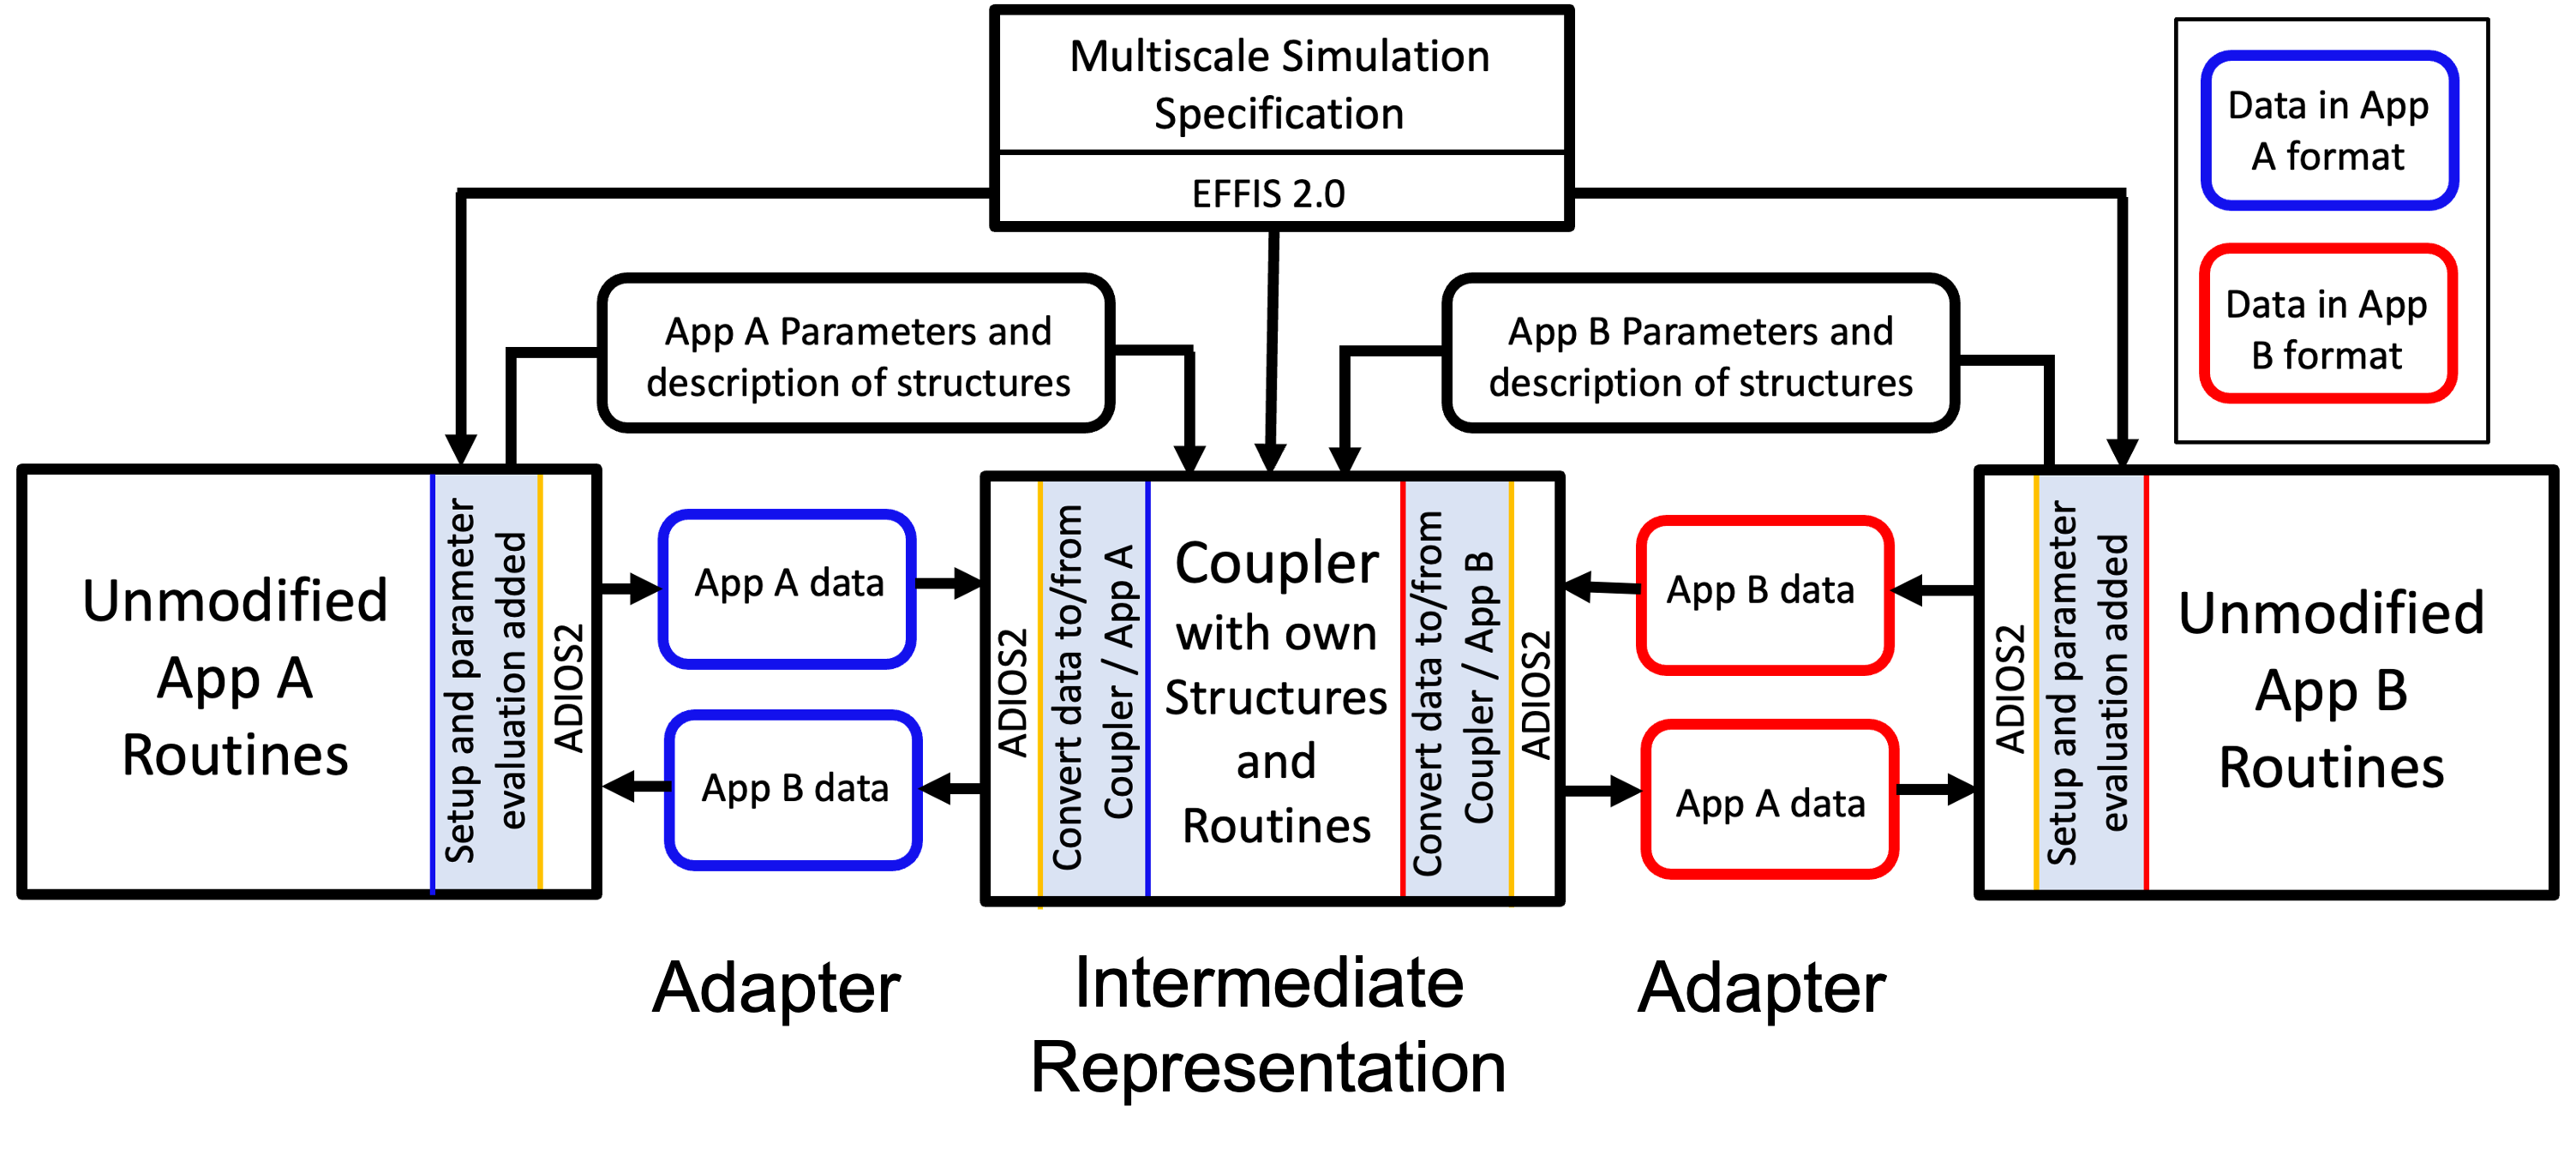
\includegraphics[width=\textwidth]{figures/coupler.png}
    \caption{Overall structure of PCMS}
    \label{fig:PCMS structure}
\end{figure}
Most multiscale and coupling libraries seek to make developing a new coupling as flexible as possible by promoting coupling setup through input files \cite{chourdakisPreCICEV2Sustainable2022,tobinAdaptiveMultiscaleSimulation2018}. We contend that developing a new coupling is done infrequently and by domain experts and is better reified in the form of source code that be partially verified through compile time checking. That said, we also intend to provide runtime configuration capabilities that can be used to quickly iterate during the development phase of new coupling pairs. To this end, we are collaborating with Manish Parashar and Philip Davis on the development of an interface to Benesh, a domain specific language and configuration layer for dynamic multimodel coupling \cite{davisBeneshProgrammingModel2020}.

Currently, PCMS only natively supports compile time coupling definitions that can provide optimizations and safety benefits over the runtime generic interfaces. Although these are compile time interfaces, it is important to understand that the coupler API design allows for an open set of field types and coordinate systems. This is enabled through a mix of compile time polymorphism and type erasure. However, the set of underlying data types (e.g., int, double, bool) are limited to datatypes that are supported in MPI and Adios2 which are used for the underlying data transport. The user can always communicate an arbitrary type by casting the data to \texttt{char}, however in this case, the user is responsible for maintaining type safety in their serialization and deserialization routines.

In the future, we expect to support two modes of runtime coupling definitions. The first makes use of a preprogrammed set of field layouts that may be able to take advantage of certain optimizations. The second, uses a schema to define all of the necessary data for coupling at runtime. Although the use of a schema provides the greatest flexibility, it gives up some level of optimization and compile time safety.

Figure \ref{fig:PCMS structure} shows the structure of a two-way coupling of App A and App B through a independent coupling server making use of PCMS. The coupler has two modes of operation: client and server mode. The client mode has a simplified interface that makes it amenable to inclusion in APIs of a variety of other programming languages. The Server interface includes operations that make use of compile time polymorphism that is hard to capture in other languages without template support. I have plans to develop a \texttt{C}/\texttt{Fortran} server interface, however it will have limitations on the types of fields/data and will either have to make use of a coupling schema (for generic field inputs), or selection of a predeveloped list of field types and will limit certain optimizations to be selected at compile time. Table \ref{tab:language support} shows the current status of language support in PCMS.

\begin{table}[]
    \centering
    \begin{tabular}{|l|c|c|}
        \hline
        Language & Client & Server \\ \hline
        C++ & \(\checkmark\) & \(\checkmark\) \\ \hline
        C & \(\checkmark\) & \\ \hline
        Fortran & \(\checkmark\) & \\ \hline
    \end{tabular}
    \caption{PCMS support for various languages in server and client mode.}
    \label{tab:language support}
\end{table}

The use of an independent coupling server in figure \ref{fig:PCMS structure} is useful in cases where both applications are unable to be linked to the libraries that support the field intermediate representation, namely ``Omega'' for unstructured meshes. Although we have developed test cases that eliminate the use of an independent coupling server, we have only performed full scale testing in a real application (XGC total-f/delta-f axisymmetric coupling) that makes use of the independent coupling server. 

PCMS supports fields and field transformations that are stored in host or device memory. However, currently Redev/Adios2 only supports host memory, so serialized fields are copied back to host memory before they are sent.

Each PCMS server and client can create a number of applications which each represent a communication pair. Each application contains a number of fields that represent the data that must coupled. In the case where an independent coupling server is used, each client will only have a single application that it communicates with, specifically the coupling server.

PCMS sends and receives fields in phases that are independent for each application. The fields that are sent and received in each phase must be identical in the server and client. Each application may only have either a send or receive phase open at a time, however this can be overlapped with phases from other applications. Depending on the \texttt{RDV} backend that is selected, no data is guaranteed to have been send/received until the phase has been completed.

The only operations that are currently available on the coupling client are to send and receive the associated fields. The coupling server additionally has gather and scatter operations. The gather operation receives fields from participating applications, performs a field transfer to the coupler's internal field representation, and combines the data from each of the participating fields into a single combined field with a user provided callback. The scatter operation splits the combined field onto the appropriate portion of the overlap domain, performs a field transfer from the internal field representation to the native field datastructures, and sends the field to the appropriate applications.

In the case of simple two-way coupling the use of gather and scatter on the server mirror the send and receive operations on the client. For more complex coupling paradigms with asymmetric send and receive phases, I have found that independently calling the field transfer routines was more convenient. This indicates that the gather and scatter API may need some degree of improvement.

\subsubsection{TODO}
Here is a nonexhaustive list of enhancements that will be needed to support a wide variety of "generalized" coupling schemes.
\begin{itemize}
    \item PCMS has a limited metadata exchange round. This needs to be to extended account for various components that are currently hardcoded such as analysis status (running/done), time stepping information, overlap domain definition, and for "schema analysis" many additional components such as shape function definition, coordinate system, etc.
    \item Control of time-stepping for implicit and explicit coupling approaches.
    \item Verification of coordinate system transformation implementation/transformation routines.
    \item Support for generalized schema field type.
    \item Refactor a "Field Layout" representation from fields to reduce the amount of field metadata exchange in initialization phase (applications tend to have many fields that share the same
    \item "input file" coupling
    \item Point to point communication protocol rather than coupling through centralized coupling server (if multiple applications are capable of performing coupling, should determine this through metadata exchange and have a protocol).
    \item GPU support for Redev
\end{itemize}

%\subsection{Communication Protocol}
%We use RDV which uses Adios2/MPI under the good. See section \ref{sec:parallel control} for more details.

\section{Parallel Control} \label{sec:parallel control}
%The control of parallel processes in PCMS (Cameron)
% the following is basically a copy-paste from https://scorec.github.io/redev/concepts/index.html
The rendezvous algorithm coordinates the information passing between pairs of coupled parallel simulations ``when processors neither know which other processors to send data to, nor which other processors will be sending data to them''~\cite{plimpton2021}.
It is used in LAMMPS~\cite{plimpton2021}, the PUMI unstructured mesh library for loading
multi-billion element meshes from file~\cite{rettenberger14} and in the Data Transfer
Toolkit~\cite{slatteryDataTransferKit2013}.

Figure~\ref{fig:redevPartition} depicts two unstructured meshes of the same domain
where information from one mesh is needed by the other but they have a
different partitioning across the same set of processes.
In Figure 4 the colored ovals depict the domain owned by a given process in
the two meshes.
Since the domains are not intersecting the Rendezvous method is used to
efficiently exchange data between the processes that do have the intersecting
portion of the domain.
A common domain partition, depicted by the red structured grid in the bottom
two figures, allows processes that own data within a given cell in grid to
'rendezvous' with the other processes that own data in that cell and perform
an exchange.

\begin{figure}
    \centering
    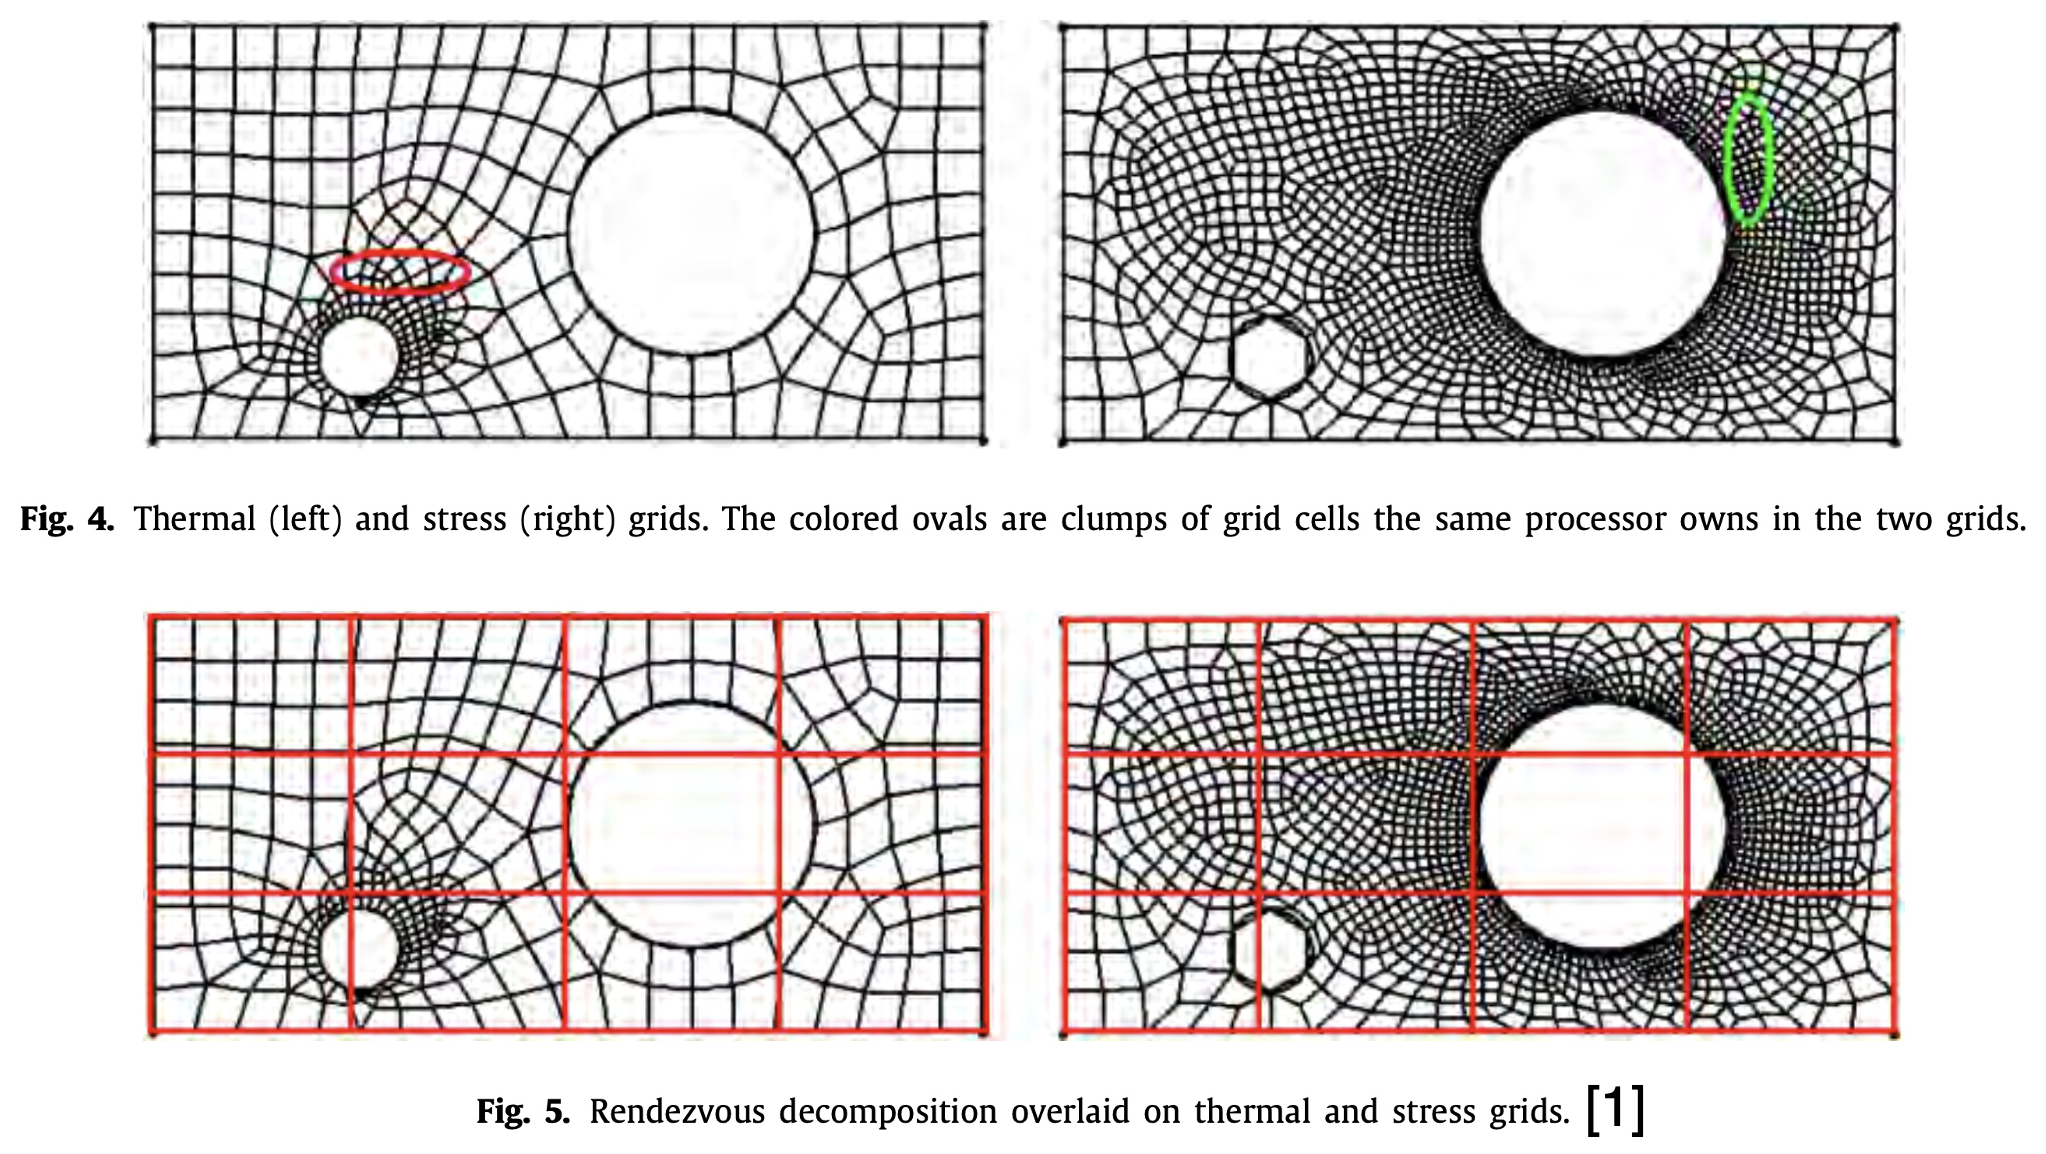
\includegraphics[width=0.75\textwidth]{figures/redevPartition.png}
    \caption{~\cite{plimpton2021}}
    \label{fig:redevPartition}
\end{figure}

The key to the Rendezvous algorithm is a partitioning of the common portion
of the domain that (1) has a relatively low memory usage and (2) supports computationally
efficient queries for membership within the partition given a entity 
within the domain (e.g., a mesh element or vertex).
The structured grid from the above figure is one possible partition that
satisfies these requirements.

The \texttt{RDV} library implements the rendezvous algorithm using \texttt{ADIOS2} data transport engines and thus enables coupling simulations that run in-memory or via files. Use of an alternative \texttt{DataSpaces} \cite{docanDataSpacesInteractionCoordination2010} backend has been demonstrated as part of the Benesh integration by Philip Davis. However, we anticipate that any demonstrated performance improvements will be contributed to \texttt{ADIOS2} and it will remain the primary communication layer as it provides the most flexibility.

\section{Field Transfer} \label{sec:field_transfer}
%Mesh to mesh transfer technologies - cover the range of methods, indicate plans and status in PCMS (Jacob)
The field transfer operations in PCMS are unique in that they are designed as algorithms that can operate generically on fields with any underlying data structures and coordinate systems. Another key aspect is that they make use of a field's native methods for query and interpolation.

To use these generic field transfer algorithms, a minimal set of customization points (free functions) must be implemented for each of the input field types. These customization points don't require any modifications to the underlying field structures, but allow for a uniform query methodology that can be used with generic algorithms.

Various field transfer methodologies exist and the choice is largely driven by cost, accuracy, and physics constraints such as the need for conservation of the underlying fields. Broadly speaking these methodologies either use a direct evaluation of the source field at the target fields's node points (interpolation/extrapolation), or solve a secondary problem to minimize some residual measure of the error in the target field (projection). Projection based methods tend to be more expensive, but make it easier to bring in physics constraints. Some authors have managed to develop conservative interpolation methods \cite{alauzetParallelMatrixfreeConservative2016}.

The field evaluation methods can further be categorized into mesh based methods, or pointwise methods. Mesh based methods use the underlying structure of the mesh whereas the pointwise methods consider the nodal points of the source data as a point cloud and impose shape functions that are independent of the discretization that is used in the solution procedures. The most common pointwise evaluation method is the use of radial basis functions (RBF) \cite{slatteryMeshfreeDataTransfer2016}. This approach is convenient in the context of coupling as it doesn't require the coupler to handle the complexities of the mesh structure. This approach has found wide success in other coupling libraries and is used to get conservative particle to cell transfers in PIC codes \cite{bungartzPreCICEFullyParallel2016,mollenImplementationHigherorderVelocity2021}. \Citeauthor{slatteryMeshfreeDataTransfer2016}, provides a comparison of radial basis functions and mesh intersection methods and concludes that the accuracy and conservative properties of RBF and mesh based methods are dependent on the geometry and field structure \cite{slatteryMeshfreeDataTransfer2016}.

Most mesh based conservative field transfer methods are based on the approach presented in \cite{jiaoCommonrefinementbasedDataTransfer2004}. In this method the fields are conservatively transferred the polyhedra that represent the intersection of the source and target meshes \cite{blanchardHighOrderAccurate2016,jaimanConservativeLoadTransfer2006,menonConservativeInterpolationUnstructured2011,farrellConservativeInterpolationVolume2011,farrellConservativeInterpolationUnstructured2009}.

Currently PCMS has an implementation for the direct evaluation (interpolation) methods that makes use of the source field's native evaluation procedures including (mesh based) nearest neighbor and Lagrange interpolation. We anticipate supporting conservative mesh based projection methods (mesh intersection) as well as point wise interpolation and conservative projection methods that make use of radial basis functions.

Note: the various field transfer methodologies work better/worse depending on the fields data and underlying geometric representation. In some cases the RBF does better w.r.t. field replication and conservation than the mesh based methods. Despite the significant increase in complexity that is added by including mesh based field transfer methods, they must be included if one is unwilling to compromise on accuracy and conservation properties in general (i.e., it is critical that the users have access to both methods and are able to test what works best for their problem of interest).

%\textbf{todo: uniform grid search methodology}

\section{Other Items to Address}
\begin{itemize}
    \item A overview of PUMIPic including design, how to use it, consideration of alternative mesh/particle relationships and ability to alter the particle data structure, etc. (Cameron).
    \begin{itemize}
      \item An introductory paragraph is here: \url{https://github.com/SCOREC/pumipic-docs/blob/d253fc0859c2e8d9d460c5b4c53b335846efb03e/pumipic_2020/introduction.tex#L81-L93}
      \item unstructured mesh data structure summary: \url{https://github.com/SCOREC/pumipic-docs/blob/d253fc0859c2e8d9d460c5b4c53b335846efb03e/pumipic_2020/data-structures.tex#L21}
      \item partitioning an unstructured mesh for PIC: \url{https://github.com/SCOREC/pumipic-docs/blob/d253fc0859c2e8d9d460c5b4c53b335846efb03e/pumipic_2020/data-structures.tex#L39}
      \item particle data structure summary: \url{https://github.com/SCOREC/pumipic-docs/blob/d253fc0859c2e8d9d460c5b4c53b335846efb03e/pumipic_2020/data-structures.tex#L210}
      \item alternative mesh/particle relationships: The PUMIPic API provides a consistent set of mesh-based particle operations across multiple implementations of the particle data structure.  Of the implementations, Sell-C-$\sigma$ [2020 PUMIPIC PAPER] and CabanaM (a implementation of the pumipic particle structure based on the ECP COPA Cabana AoSoA~\cite{Slattery2022}) have been demonstrated to provide high performance for PIC simulations with hundreds, or more, of particles per element [XGCM PAPER].  Methods that utilize many fewer particles per element, such as the material point method or PIC for impurity tracking, may want to avoid the need to explicitly store particles on a per element basis while still supporting the ability to operate on particles at the element level.  For this use case a new structure, DPS, is under development. Relative to Sell-C-$\sigma$ and CabanaM, it is designed to have a very fast update of the particle-to-element association at the expense of non-coalesced memory access when looping over elements and the particles within them. The expectation is that this trade-off will net in increased overall performance for these applications.  Critically, these performance studies can be performed without disrupting application code as all of the aforementioned particle data structures use the same PUMIPic APIs.
    \end{itemize}
    \item Supporting unstructured meshes and fields on CPU/GPUs - functionalities, tools, and adapativity (Cameron)
    \begin{itemize}
      \item PUMI (\url{https://www.scorec.rpi.edu/reports/view_report.php?id=666}) major features:
      \begin{itemize}
        \item Scaled to millions of processes on meshes with billions of elements
        \item Support for parallel adaptation of straight sided, curved and semi-structured boundary layer like meshes.
        \item Parallel field interface for defining physical fields, their distribution across the mesh, and basis/shape functions for supporting field transfer during mesh adaptation and estimating errors to drive mesh adaptation.
        \item CPU only
      \end{itemize}
      \item Omega\_h (\url{https://www.scorec.rpi.edu/REPORTS/2016-25.pdf}) major features:
      \begin{itemize}
        \item On a single Summit V100 Omega\_h GPU adaptation to an isotropic size field generated by the PUMI-MFEM RF analysis from 260k to 1.4M tets completes in 4.06 seconds.  On 16 processes (of the 24 available) on an AMD EPYC 7451 (1st generation) CPU PUMI completes adaptation in 20.6 seconds.  Figure~\ref{fig:rfAdapt} depicts the adapted mesh. 
        %from email subject= "Re: Start at the adaptive presentation for SIAM PP2022" date=2/14/22, 09:39
        %see pp22 slides, 'omegahMfem', slide title "2nd adapt for ICRF antenna of the large plasma device"
        \item Parallel mesh adaptation on GPU and CPU - ran on AMD, Intel and Nvidia GPUs
        \item GPU aware parallel field interface for defining physical fields and their distribution is being developed.  The interface follows the concepts defined by PUMI but using array-based APIs for efficient execution on GPUs.  The interface is implemented with Kokkos or ECP COPA-Cabana.  Users who need runtime sizing of the data associated with each mesh entity (e.g., the number of dofs per vertex for a given field) would select the Kokkos implementation (The Cabana AoSoA only supports compile-time sizing) at the possible expense of some performance. %https://github.com/SCOREC/meshFields/tree/main/src
        \item Supports simplicies (triangles and tets) only.
      \end{itemize}
    \end{itemize}
\end{itemize}

\begin{figure}[!h]
    \centering
    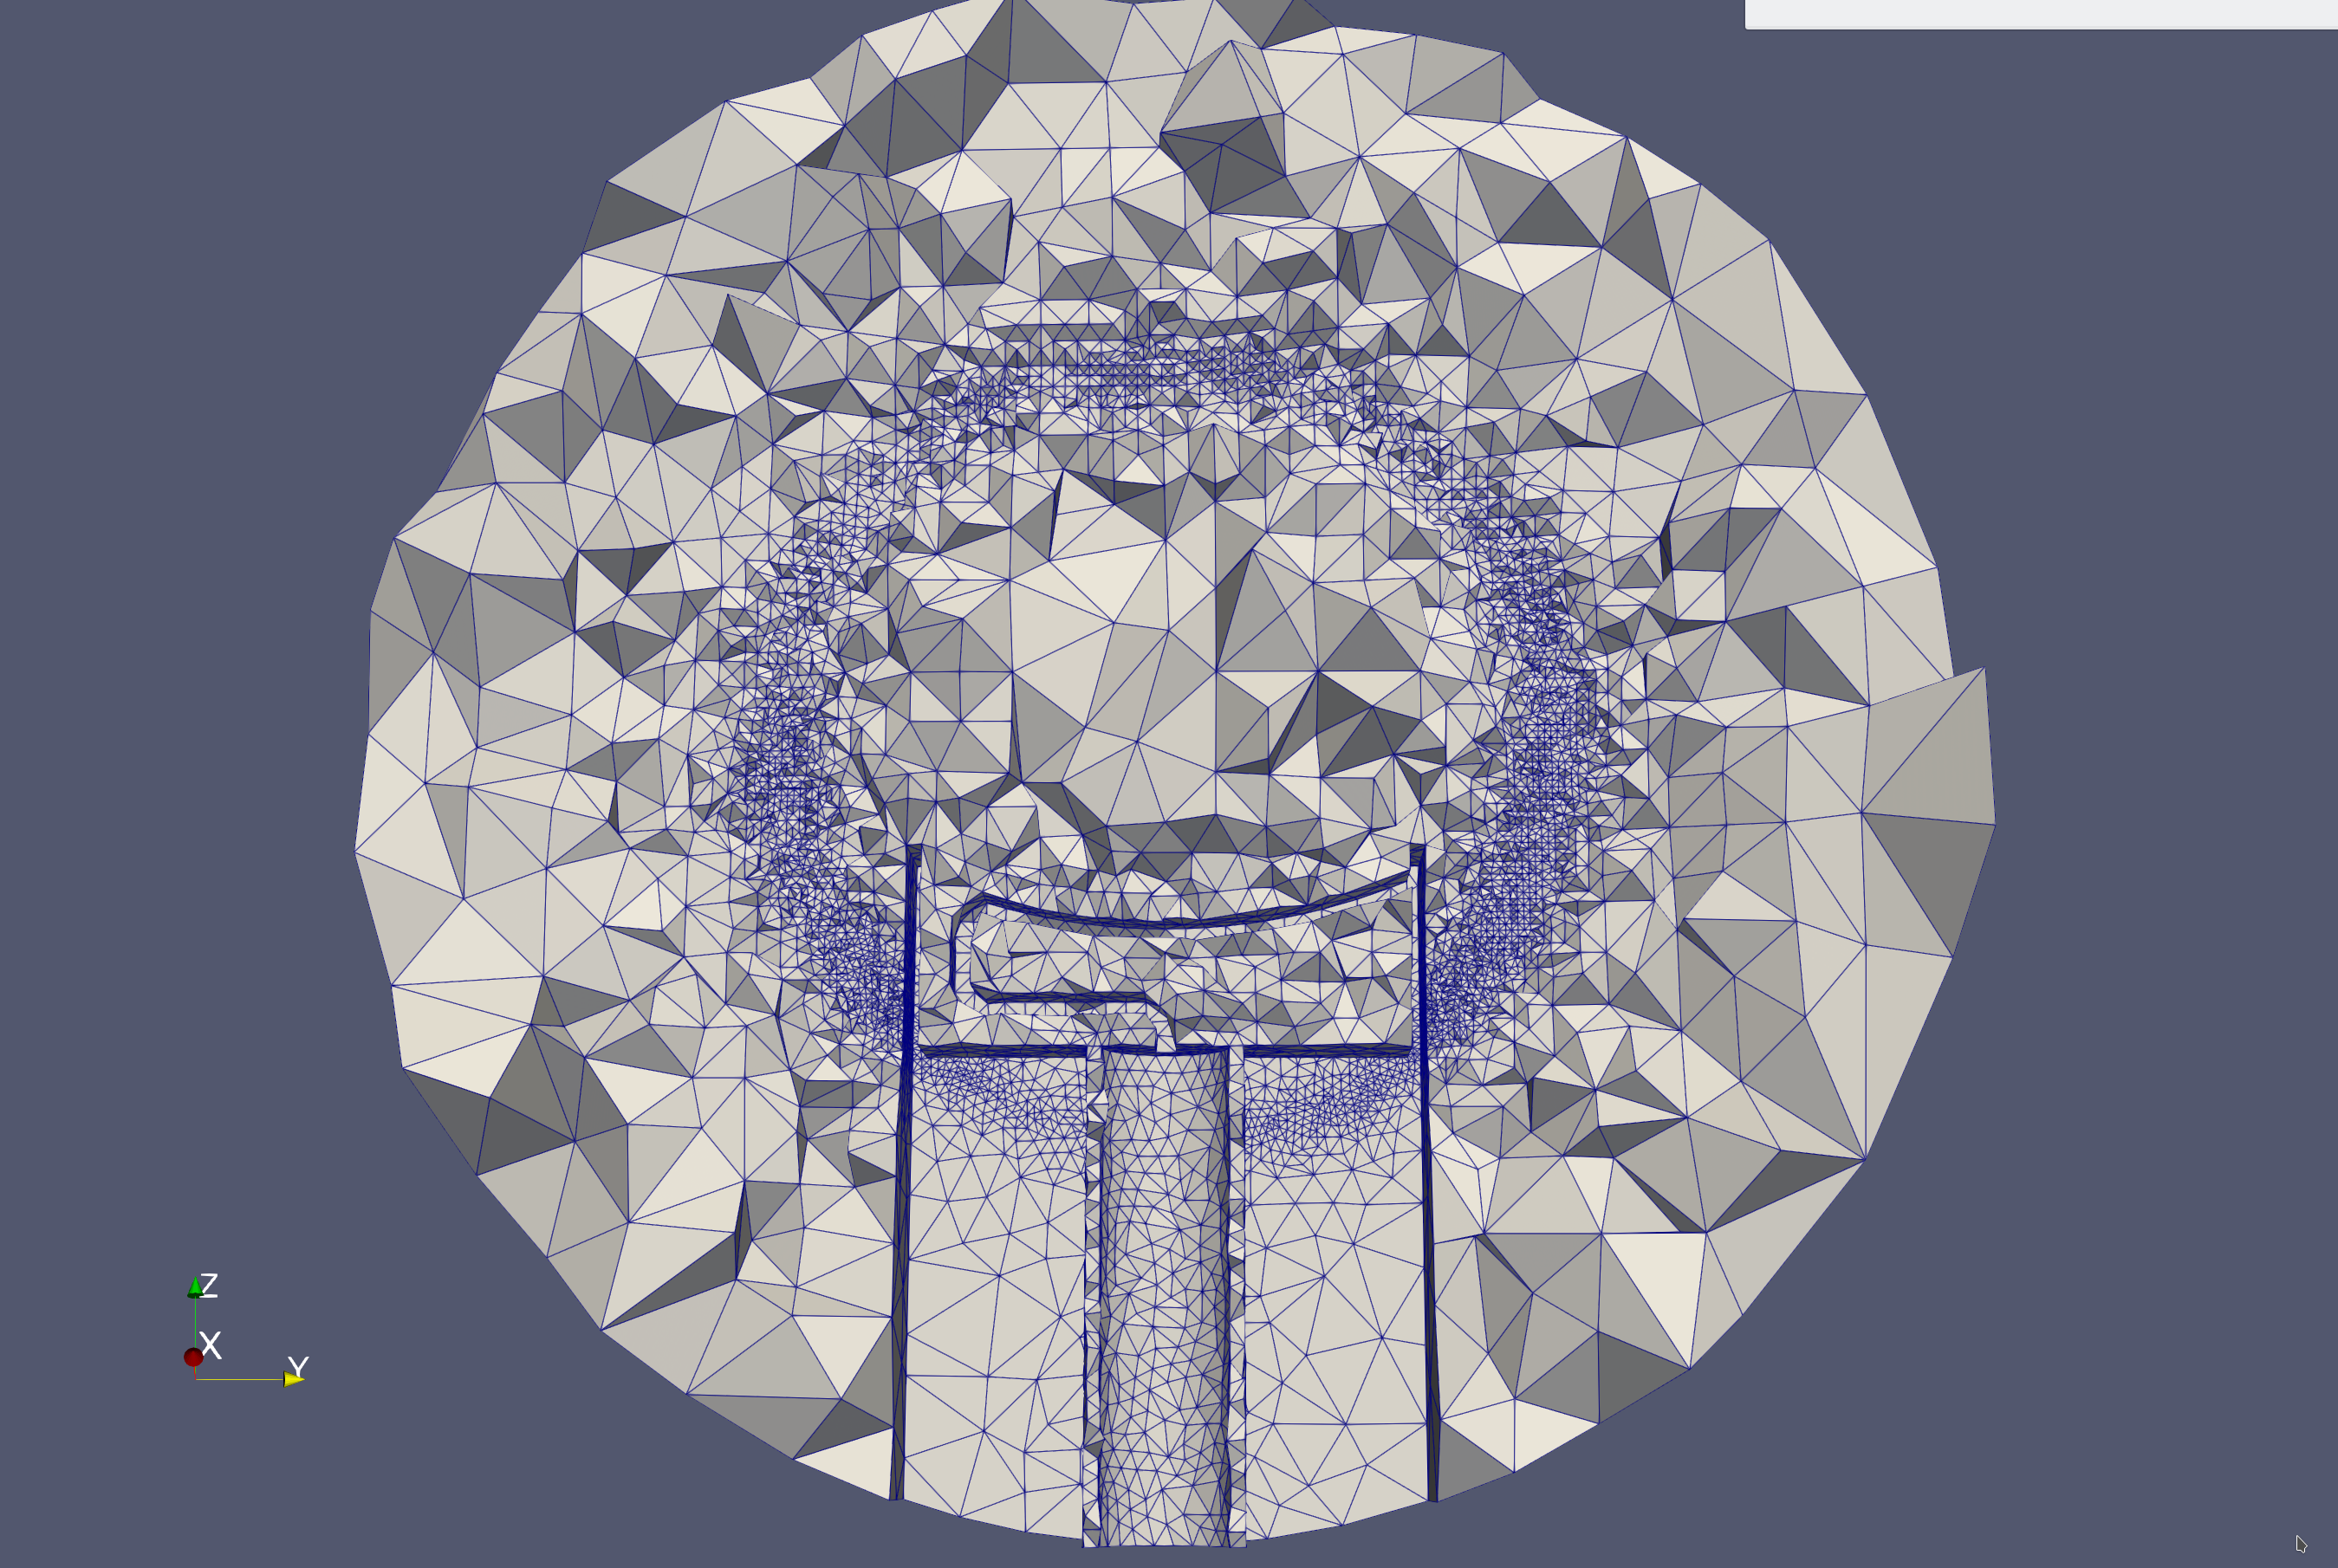
\includegraphics[width=0.75\textwidth]{figures/omegah_adapted_graded.png}
    \caption{Omega\_h adapted mesh on the isotropic size field from a PUMI-MFEM RF analysis.}
    \label{fig:rfAdapt}
\end{figure}

\printbibliography
\end{document}
